\section{Cross-Model Construction and Scripted Execution}
\label{sec:extended}

\subsection{A Separate One-Sentence Corpus}
The August 25 archive adds eight recorded model identifiers and three shared
one-sentence prompts: a city taxing spoken promises by weight, a railway
greenhouse allocating access through crop-care obligations, and a courthouse
rebuilding a shoreline from confiscated objects. This later pipeline requests
12 agents and four player slots. We re-audit its 24 generation outcomes
separately from the earlier ten-brief comparison: the prompt set, implementation,
and available models changed, so their scores are not pooled.

Seventeen of 24 trials yield complete artifacts, with nine first-pass
completions. Five models complete all three prompts; Gemini 3.5 Flash Lite
and GPT-5.6 Terra each complete only the first, and GPT-5.6 Luna completes none.
Table~\ref{tab:extended-audit} retains every failure. These are recorded API
identifiers, not guarantees of immutable provider snapshots. One generation
per model--prompt cell supports a coverage diagnosis, not a stable model ranking.
Although the archive calls the suite hidden/confirmatory, it lacks a
pre-execution immutable registration, and some scoring and retry policies
were revised after development runs. We treat it as retrospective evidence.

\subsection{What the Longer Harness Actually Measures}
Seven first-prompt artifacts support three repeated 24-round trajectories
each. The harness makes six calls per trajectory, at rounds 1, 5, 9, 13, 17,
and 21; each call plans 12 actions over four rounds. Its planner observes
summaries of \emph{all} agents and recent events. It is a centralized
multi-character policy, distinct from the locally observed agents in
Section~\ref{sec:method}. Scripted requests, an invalid transfer, a resource
shock, and a cross-room request probe execution. The prompt explicitly asks
for thread continuation, legal recovery, and human follow-through; these
behaviors cannot be claimed as spontaneous emergence or participant engagement.

The 21 trajectories contain 1,512 attempted model actions, of which 1,365
succeed (90.3\%). Among successful actions, 398 (29.2\%) record an inventory
or location mutation. Among 314 approved proposals, 150 (47.8\%) declare at
least one non-speech effect; status-only effects count in this latter measure.
These denominators address different questions and are not interchangeable.
Figure~\ref{fig:extended-runtime} reports model-specific counts and repeat
ranges instead of a weighted quality score.

\begin{figure*}[t]
\centering
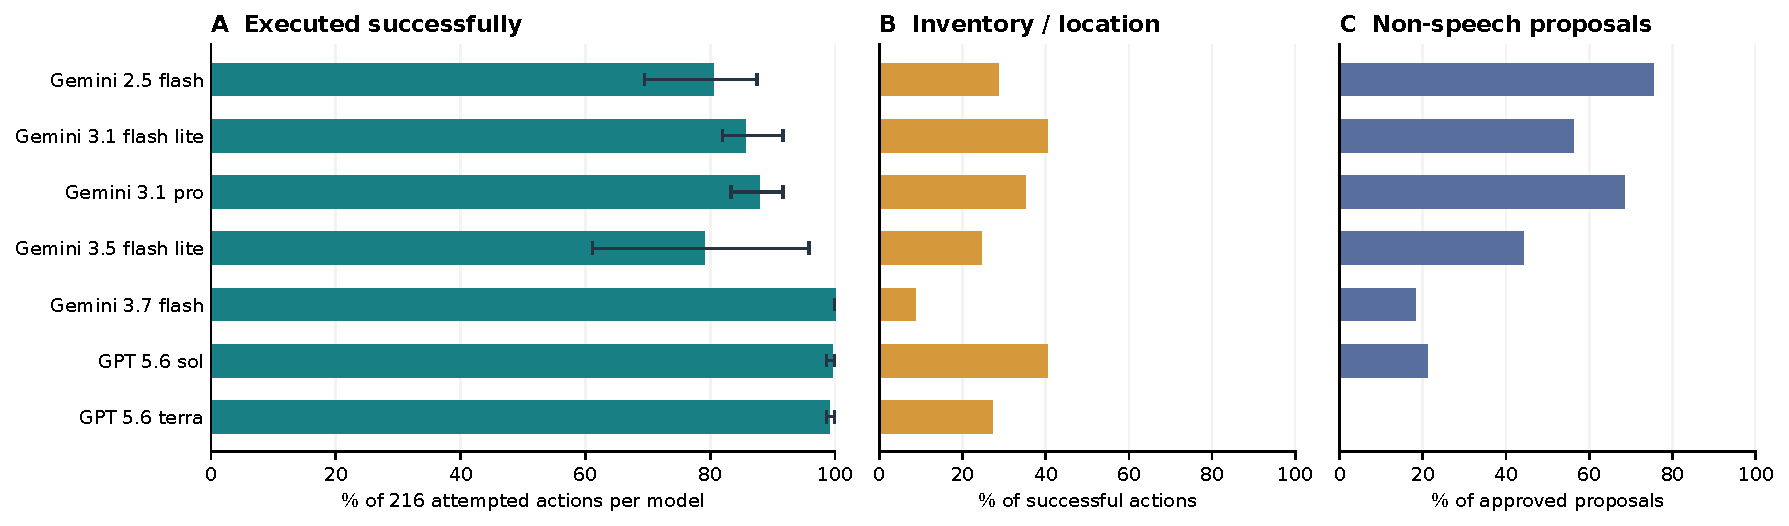
\includegraphics[width=\textwidth]{figures/extended_runtime_audit.pdf}
\caption{\paneltitle{Successful execution does not ensure rich consequences.}
Seven generated worlds, each with three 24-round centralized-policy runs.
(A) Success per attempted action; whiskers are the minimum and maximum over
three runs, not confidence intervals. (B) Inventory/location mutations among
successful actions. (C) Non-speech effects among approved proposals, including
status changes. All comparisons couple a model with its own generated world;
they do not isolate policy capability on identical environments.}
\label{fig:extended-runtime}
\end{figure*}

\subsection{Failure Modes and Evidence Boundaries}
Gemini 3.7 Flash succeeds on all 216 attempts, but only 19 successes change
inventory or location and only four of 22 approved proposals have non-speech
effects. Terra's 18 approved proposals are all speech-only, despite 214/216
successful actions. Conversely, Gemini 2.5 Flash has 42 failed attempts but
34/45 approved proposals with non-speech effects. These observations motivate
reporting \emph{what changed} alongside whether an action executed, consistent
with analytical trajectory evaluation \cite{agentboard}.

All 147 failed model actions and all 21 scripted invalid transfers leave their
recorded state hashes unchanged. Final-state serialization round trips match
in 21/21 runs; this checks serialization, not recovery after a process crash.
Of 1,021 recorded relationship updates, 1,013 have the same
$(\Delta\mathrm{trust},\Delta\mathrm{affection},\Delta\mathrm{fear})=(4,2,0)$.
The custom-action handler supplies exactly this default for non-aggressive
actions. Thus rising relationship values in this harness largely reflect
execution rules rather than independently demonstrated social development.
Appendix~\ref{app:extended} provides the full audit and replication boundaries.
